%% 
%% Copyright 2019-2021 Elsevier Ltd
%% 
%% This file is part of the 'CAS Bundle'.
%% --------------------------------------
%% 
%% It may be distributed under the conditions of the LaTeX Project Public
%% License, either version 1.2 of this license or (at your option) any
%% later version.  The latest version of this license is in
%%    http://www.latex-project.org/lppl.txt
%% and version 1.2 or later is part of all distributions of LaTeX
%% version 1999/12/01 or later.
%% 
%% The list of all files belonging to the 'CAS Bundle' is
%% given in the file `manifest.txt'.
%% 
%% Template article for cas-sc documentclass for 
%% single column output.

\documentclass[a4paper,fleqn]{cas-sc}
% Use to make nonmenclature
\usepackage{framed} % Framing content

\usepackage{multicol} % Multiple columns environment
\usepackage{amsmath}
\usepackage{nomencl} % Nomenclature package

\makenomenclature

\setlength{\nomitemsep}{-\parskip} % Baseline skip between items

\renewcommand*\nompreamble{\begin{multicols}{2}}

\renewcommand*\nompostamble{\end{multicols}}
% If the frontmatter runs over more than one page
% use the longmktitle option.

%\documentclass[a4paper,fleqn,longmktitle]{cas-sc}

\usepackage[numbers]{natbib}
%\usepackage[authoryear]{natbib}
%\usepackage[authoryear,longnamesfirst]{natbib}

%%%Author macros
\def\tsc#1{\csdef{#1}{\textsc{\lowercase{#1}}\xspace}}
\tsc{WGM}
\tsc{QE}
%%%

% Uncomment and use as if needed
%\newtheorem{theorem}{Theorem}
%\newtheorem{lemma}[theorem]{Lemma}
%\newdefinition{rmk}{Remark}
%\newproof{pf}{Proof}
%\newproof{pot}{Proof of Theorem \ref{thm}}

\begin{document}
\let\WriteBookmarks\relax
\def\floatpagepagefraction{1}
\def\textpagefraction{.001}

% Short title
\shorttitle{}    

% Short author
\shortauthors{B.T. Rawlins et el.}  

% Main title of the paper
\title [mode = title]{Validation of an integrated data-driven surrogate model and a thermo-hydraulic network based model to determine boiler operational loads using a fully connected mixture density network}  

% Title footnote mark
% eg: \tnotemark[1]
%\tnotemark[<tnote number>] 

% Title footnote 1.
% eg: \tnotetext[1]{Title footnote text}
%\tnotetext[<tnote number>]{<tnote text>} 

% First author
%
% Options: Use if required
%\author[1,3]{Author Name}[type=editor,
%       style=chinese,
%       auid=000,
%       bioid=1,
%       prefix=Sir,
%       orcid=0000-0000-0000-0000,
%       facebook=<facebook id>,
%       twitter=<twitter id>,
%       linkedin=<linkedin id>,
%       gplus=<gplus id>]

\author[1]{B.T. Rawlins}

% Corresponding author indication
\cormark[1]
\cortext[1]{Corresponding author}
% Footnote of the first author
%\fnmark[<footnote mark no>]

% Email id of the first author
\ead{rwlbra001@myuct.ac.za}

% URL of the first author
%\ead[url]{<URL>}

% Credit authorship
% eg: \credit{Conceptualization of this study, Methodology, Software}
\credit{Methodology, Software, Validation, Formal analysis, Investigation,Writing original draft, Visualization.}

% Address/affiliation
\affiliation[1]{organization={Department of Mechanical Engineering, Applied Thermal-Fluid Process Modelling Research Unit, University of Cape Town},
            addressline={Library Road, Rondebosch}, 
            city={Cape Town},
%          citysep={}, % Uncomment if no comma needed between city and postcode
            postcode={7701}, 
            %state={},
            country={South Africa}}

\author[2]{Ryno Laubscher}[]

% Footnote of the second author
%\fnmark[2]

% Email id of the second author
\ead{rlaubscher@sun.ac.za}
% URL of the second author
%\ead[url]{}
% Credit authorship
\credit{Writing review \& editing, Methodology, Resources, Conceptualization.}
% Address/affiliation
\affiliation[2]{organization={Department of Mechanical Engineering, Stellenbosch University},
            addressline={Banghoek Road, Stellenbosch}, 
            %city={Stellenbosch},
%          citysep={}, % Uncomment if no comma needed between city and postcode
            postcode={7600}, 
            %state={},
            country={South Africa}}
% Footnote text
%\fntext[1]{}
% For a title note without a number/mark
%\nonumnote{}
\author[1]{Pieter Rousseau}
% Email id of the second author
\ead{pieter.rousseau@uct.ac.za}
% Credit authorship
\credit{Writing review \& editing, Resources, Conceptualization}

% Corresponding author text


% Here goes the abstract
\begin{abstract}
A data-driven surrogate model is proposed for a 620$MW_e$ sub-critical power boiler. The surrogate model was developed using computational fluid dynamic (CFD) simulation data. The simulation data covered a varied range of inputs.
\end{abstract}

% Use if graphical abstract is present
%\begin{graphicalabstract}
%\includegraphics{}
%\end{graphicalabstract}

% Research highlights
\begin{highlights}
\item Development of mixture density network using simulation data.
\item Model based on validated CFD model of a 620 $MW_e$ sub-critical boiler.
\item Surrogate model prediction errors are below 10\%.
\end{highlights}

% Keywords
% Each keyword is seperated by \sep
\begin{keywords}
Mixture density network \sep Surrogate modelling \sep Boiler operation \sep 
\end{keywords}

\maketitle

% Main text
\section{Introduction}\label{intro}

The use of neural networks for the modelling of energy systems has been awesome. Optimization of a plant is extremely fun. Using the surrogate model development the model can be developed


\newpage
\begin{table*}[!t]   

\begin{framed}

\nomenclature{$abbreviation$}{explanation for the abbreviation}
\nomenclature{$CFD$}{Computational Fluid Dynamics}
\nomenclature{$u,\,\,\,[m/s]$}{Directional velocity}
\nomenclature{$p,\,\,\,[Pa]$}{Pressure}
\nomenclature{$E,\,\,\,[J/kg]$}{Total energy}
\nomenclature{$Y_k,\,\,\,[kg/kg]$}{Mass fraction of species $k$}
\nomenclature{$T_g,\,\,\,[K]$}{Gas temperature}
\nomenclature{$\lambda,\,\,\,[W/mK]$}{Thermal conductivity}
\nomenclature{$\mu,\,\,\,[Pa.s]$}{Viscosity}
\nomenclature{$S,\,\,\,[kg/m^3]$}{Mass source term}
\nomenclature{$S_m,\,\,\,[N/m^3]$}{Momentum source term}
\nomenclature{$S_h,\,\,\,[W/m^3]$}{Energy source term}
\nomenclature{$S_k,\,\,\,[kg/m^3]$}{Species source term}
\nomenclature{$J_k,\,\,\,[kg/m^3]$}{Diffusion flux of species $k$}
\nomenclature{$\rho,\,\,\,[kg/m^3]$}{Gas density}
\nomenclature{$\rho_{eff},\,\,\,[kg/m^3]$}{Effective density}
\printnomenclature

\end{framed}

\end{table*}
% Numbered list
% Use the style of numbering in square brackets.
% If nothing is used, default style will be taken.
%\begin{enumerate}[a)]
%\item 
%\item 
%\item 
%\end{enumerate}  

% Unnumbered list
%\begin{itemize}
%\item 
%\item 
%\item 
%\end{itemize}  

% Description list
%\begin{description}
%\item[]
%\item[] 
%\item[] 
%\end{description}  

% Figure
%\begin{figure}%[<options>]
	%\centering
	%	\includegraphics[<options>]{}
	 % \caption{}\label{fig1}
%\end{figure}


%\begin{table}[<options>]
%\caption{}\label{tbl1}
%\begin{tabular*}{\tblwidth}{@{}LL@{}}
%\toprule
 % &  \\ % Table header row
%\midrule
 %& \\
 %& \\
 %& \\
% & \\
%\bottomrule
%\end{tabular*}
%\end{table}

% Uncomment and use as the case may be
%\begin{theorem} 
%\end{theorem}

% Uncomment and use as the case may be
%\begin{lemma} 
%\end{lemma}

%% The Appendices part is started with the command \appendix;
%% appendix sections are then done as normal sections
%% \appendix

\section{Applicable machine learning theory}

\section{Data generation}
A steady-state multiphase non-thermal equilibrium CFD model was used to generate the target data, which was subsequently used for training/development of an appropriate surrogate model.

\subsection{CFD model setup}
The current study makes use of the commercial CFD software package ANSYS\textsuperscript{\textregistered} Fluent 2019 R3 to resolve the fluid flow, heat transfer and combustion processes for a 620$MW_e$ utility scale coal fired boiler. The computational domain is modelled on a symmetry plane half way through the depth of the boiler. Figure \ref{fig_cfd_geom_bc} highlights the computational domain and defines the important boundary conditions.\\ 

\begin{figure}[h!]
	\centering
		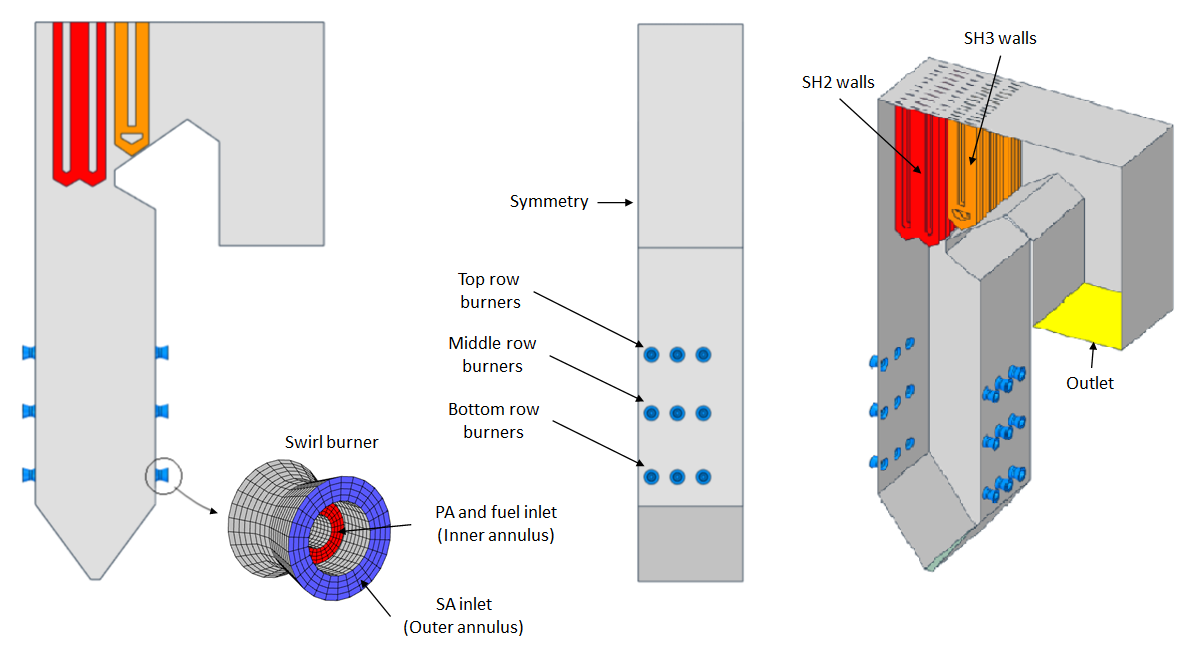
\includegraphics[scale=0.5]{CFD_GEOMETRY}S
	  \caption{CFD model geometry and boundary condition descriptions.}\label{fig_cfd_geom_bc}
\end{figure}

The general conservation equations, which include, continuity, momentum, energy and species, were solved using a Eulerian approach. The subsequent equations are stated in Equation (\ref{eqn_cfd}).

\begin{flalign} \label{eqn_cfd}
&\frac{\partial}{\partial x_{i}}(\rho \bar{u}_{i})=S \nonumber &&\\
&\frac{\partial}{\partial x_{i}}(\rho_{eff} u_{i}u_{j})+\frac{\partial \overline{p}}{\partial x_{j}}=\frac{\partial}{\partial x_{i}}\left[\mu\left\{\frac{\partial u_{j}}{\partial x_{i}}+\frac{\partial u_{i}}{\partial x_{j}}-\frac{2}{3}\delta_{ij}\frac{\partial u_{i}}{\partial x_{i}}\right\}\right]+\frac{\partial}{\partial x_{i}}(-\rho\overline{u_{i}^{'}u_{j}^{'}})+S_m \nonumber &&\\
&\frac{\partial }{\partial x_{i}} (u_{i}[\rho E+p])=\frac{\partial }{\partial x_{j}}\left[\lambda\frac{\partial T_{g}}{\partial x_{j}}\right] +S_{h} &&\\
&\frac{\partial}{\partial x_{i}}(\rho u_{j}Y_{k})=-\frac{\partial}{\partial x_{j}}(\vec{J_{k}})+ \sum_r R_{j,r} + S_{k} \nonumber && 
\end{flalign}

The resolution of the Reynolds stress term found in the momentum equation, $-\rho\overline{u_{i}^{'}u_{j}^{'}}$, was approximated using the Boussineq equation \citep{Versteeg2007}. In the present study the realizable k-$\varepsilon$ turbulence model was utilized to address the turbulence closure problem, this model was selected for its applicability in modelling the effects of coal-fired swirl burners \citep{Modlinski2010}.\\

The P1 radiation model was used to resolve the radiative field in the domain. Particle transport was modelled using a multiphase approach, further details on the approach are provided in the validation study of Rawlins et al \citep{Rawlins2021}. The combustion follows a four step sequential process, beginning with the heating and evaporation of the moisture present in the fuel, followed by the devolatilization process where the volatiles are liberated from the solid particle, succeeded by the phenomena of char burnout, and finally the gas phase reactions would commence. The char oxidation reaction product species was set to that of carbon monoxide ($CO$). For the gas-phase reactions the turbulence-chemistry interaction was approximated using the eddy dissipation model (EDM). A summary of the combustion equations and constants are provided in Table \ref{tbl_combust}.\\

\begin{table}[h!]
\caption{Summary of combustion models and constants used in the CFD model}\label{tbl_combust}
\begin{tabular*}{\tblwidth}{p{0.325\textwidth}p{0.35\textwidth}p{0.25\textwidth}}
\toprule
Model & Equation/s & Constant/s\\
\midrule
\multicolumn{3}{l}{\textit{Devolatilization}} \\ % Table header row
Single rate kinetic model &$\frac{dm_{vol}}{dt} = R_{vol}(m_{0,vol}-m_{vol})$,  & $A_{vol} = 2\times10^5 [s^{-1}]$, \\
& $R_{vol} = A_{vol}exp\left(\frac{E_{a,vol}}{RT_p}\right)$ & $ E_{a,vol} = 6.7\times10^7 [J/kmol]$ - \cite{Sheng2004} \\
\multicolumn{3}{l}{\textit{Char oxidation}} \\
Diffusion/kinetic - \citep{Baum1971} & $\frac{dm_{char}}{dt} = -A_p p_{O_{2}} \frac{R_{diff}R_c}{R_{diff} + R_c}$,  & $A_{c} = 0.0053 [kg/m^2sPa]$, \\
& $R_{c} = A_{c}exp\left(\frac{E_{a,c}}{RT_p}\right)$,  & $E_{a,c} = 8.37\times10^7 [J/kmol]$ - \cite{Sheng2004} \\
& $R_{diff} = \frac{5\times10^{-12}}{d_p} \left(\frac{T_g+T_p}{2}\right)^{0.75}$&\\
\multicolumn{3}{l}{\textit{Gaseous reactions of volatiles and $CO$}} \\
Eddy dissipation model - \cite{Ansys} & $R_{k,r,P} =\vartheta_{k,r}M_{w,k}AB\rho\frac{\varepsilon}{k}min\left(\frac{\sum_{p} Y_p}{\sum_{j}\vartheta_{j,r}M_{w,j}}\right)$, $R_{k,r,R} =\vartheta_{k,r}M_{w,k}A\rho\frac{\varepsilon}{k}min\left(\frac{Y_R}{\varepsilon_{R,r}M_{w,R}}\right)$ & $A=4.0$, $B=0.5$\\
\bottomrule
\end{tabular*}
\end{table}

The simulations were solved using the SIMPLE pressure–velocity coupling scheme. The pressure term was discretized using the PRESTO! scheme. Momentum, species and energy equations were discretized using the second-order upwind scheme and the turbulent kinetic energy and dissipation rate using the first-order upwind scheme. The numerical mesh was generated using quadrilateral elements consisting of 6 million cells.  The convergence criteria for the simulation model was set to $1\times10^{-3}$ for the continuity equation, $1\times10^{-4}$ for the velocity equations, $1\times10^{-6}$ for the remaining transport equations, and $1\times10^{-4}$ for monitored key parameters.

\subsection{Simulated dataset}
As previously mentioned the aim this study is to illustrate the use of a data-driven surrogate model, integrated with a 1D process model, to predict the heat loads to the various heat exchanging components, the flue-gas composition and exit gas temperatures for a utility scale boiler using various high-level inputs. The inputs include the the following, the excess air ratio per burner, the total mill flowrate for the six mills in operation, the average steam temperatures for the platen and final superheaters, the fouling resistance for the platen and final superheaters, the composition of ash and moisture of the fuel and the gross calorific value of the fuel. Thus the input field has a dimensionality of $d_{input}=14$.\\

A design of experiments (DOE) was conducted to generate a set of 180 simulation cases to obtain a representative set of results. The various model input ranges used in the DOE are given in Table \ref{tbl_doe}. The ranges where selected to cover a wide range of operational loads with maximum continuous ratings (MCR) between 100\% and 30\%.

\begin{table}[h!]
\caption{Design of experiments input ranges for  simulations}\label{tbl_doe}
\begin{tabular*}{\tblwidth}{p{0.5\textwidth}p{0.15\textwidth}p{0.15\textwidth}p{0.15\textwidth}}
\toprule
 Input variable& Min& Max& Units \\ % Table header row
\midrule
 Total fuel flow rate for mills 1 to 6 & 39.5 & 120.2 & $kg/s$ \\
 Excess air & 1.155 & 1.401 & $\%$\\
 Fuel proximate analysis moisture mass fraction, $Y_{H_2O}$ & 0.025 & 0.085 & $kg/kg$ \\
 Fuel proximate analysis ash mass fraction, $Y_{ash}$  & 0.259 & 0.559 & $kg/kg$ \\
 Platen SH fouling thermal resistance, $R_{platen}$  & 0.004 & 0.007 & $m^2K/W$ \\
 Final SH fouling thermal resistance, $R_{final}$  &0.01 & 0.017 & $m^2K/W$ \\
\bottomrule
\end{tabular*}
\end{table}

\section{Model development}
The present work makes use of two types of machine learning models, namely a standard artificial neural network (ANN) and a mixture density designated model connected to a standard ANN (MDN-ANN). The following section will discuss the hyper parameter tuning and final selected model configuration. The programming language Python 3.7.8 and the Tensorflow machine learning libraries were utilized in the present study. 
\subsection{Model configuration}


\subsection{Hyper parameter tuning \& final model selection}

table of NN and MDN data comparison for tuning

\clearpage
\begin{table}[h!]
\caption{Hyper-parameter search space for fully connected NN and MDN models}\label{tbl_tuning}
\begin{tabular*}{\tblwidth}{p{0.5\textwidth}p{0.24\textwidth}p{0.24\textwidth}}
\toprule
 Parameter& NN search space & MDN search space \\ % Table header row
\midrule
 Number of distributions & - & 2,3,4  \\
 Number of layers & 2,3,4 & 2,3,4\\
 Number of neurons per layer & 10, 40, 80, 100  & 10, 40, 80, 100\\
 Learning rates & 1e-3, 1e-4, 1e-5 &  1e-3, 1e-4, 1e-5   \\
 Mini batch sizes  & 16, 32, 64 & 16, 32, 64  \\
\bottomrule
\end{tabular*}
\end{table}
Table \ref{tbl_tuning} highlights the hyper-parameter search spaces for both the ANN and ANN-MDN model. The ANN-MDN has an added parameter namely the number of additional distributions the ANN-MDN would fit to the output data. \\

The hyper-parameter search was conducted in a sequential manner with the number of layers and neurons per layer being the initial step, after which the learning rates were varied, followed by the batch sizes. The ANN-MDN hyper-parameter tuning was conducted in a similar manner only that an additional step is required to establish the best amount of distributions.

\begin{table}[h!]
\caption{ANN model selection results}\label{tbl_tuning}
\begin{tabular*}{\tblwidth}{p{0.5\textwidth}p{0.24\textwidth}p{0.24\textwidth}}
\toprule
 Parameter& NN search space & MDN search space \\ % Table header row
\midrule
 Number of distributions & - & 2,3,4  \\
 Number of layers & 2,3,4 & 2,3,4\\
 Number of neurons per layer & 10, 40, 80, 100  & 10, 40, 80, 100\\
 Learning rates & 1e-3, 1e-4, 1e-5 &  1e-3, 1e-4, 1e-5   \\
 Mini batch sizes  & 16, 32, 64 & 16, 32, 64  \\
\bottomrule
\end{tabular*}
\end{table}

\section{Results and discussion}
\subsection{Multiple load validation}

Validation includes the use of integrating the surrogate model with a network based-process model of the water/steam side of the utility boiler under investigation. A C\# script is used to access the Python API available in the process modelling software, Flownex SE\textsuperscript{\textregistered} 2021. This allows for predictions to be made using the trained MDN model. The most probable predictions are retrieved using the surrogate model script and transferred to the respective process model components. A schematic of the surrogate and process models integration is provided in Figure \ref{fig_int_model}.

\begin{figure}[h!]
	\centering
		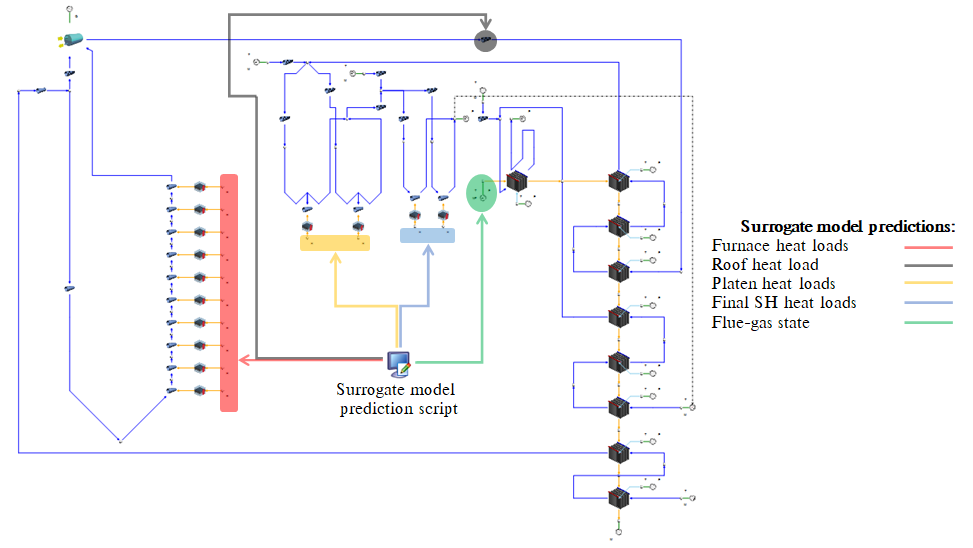
\includegraphics[scale=0.65]{INTEGRATED_MODEL}S
	  \caption{Schematic of integrated surrogate and network based process model}\label{fig_int_model}
\end{figure}

Measured plant data for a 100\%, 81\% and 60\% MCR load ratings was made available and is to be used compare the accuracy of the integrated model.
\subsection{Utility boiler response to poor fuel combustion}
The fuel quality is an important factor when determining the 
Fuels with total moisture contents exceeding 
The following results illustrate the effects poor quality fuel has on the case studies boiler operational. The study made use of the developed surrogate model to investigate the steady state operation of the boiler burning poor quality coal.  
In this section the results of a study conducted  
\section{Conclusion}

The present work has shown it is possible
% To print the credit authorship contribution details
\printcredits

%% Loading bibliography style file
%\bibliographystyle{model1-num-names}
\bibliographystyle{cas-model2-names}

% Loading bibliography database
\bibliography{ML_paper}

% Biography
\bio{}
% Here goes the biography details.
\endbio

%$\bio{pic1}
% Here goes the biography details.
%\endbio

\end{document}


